\documentclass[a4paper,12pt,oneside]{extbook}
\usepackage[english,russian]{babel}
\usepackage{fontspec}
\usepackage{subcaption}
\usepackage{graphicx}
\usepackage{indentfirst}
\usepackage{caption}
\usepackage{wrapfig}
\usepackage{xcolor,soul,lipsum}
\usepackage{amsmath}
\usepackage{amsthm}
\usepackage{hyperref}
\usepackage{enumitem} % no item sep in list
\usepackage[explicit]{titlesec}
\usepackage{amssymb}
\usepackage{titletoc}
\usepackage{tocvsec2}
\usepackage{tocloft}
\usepackage[b]{esvect}
\usepackage{mdframed}
\usepackage{textcomp}
\usepackage{multicol}
\usepackage{minted}
\usepackage[%
    left=0.8in,%
    right=0.8in,%
    top=0.8in,%
    bottom=1in,%
]{geometry}%

\newmdenv[
    linewidth=2pt,
    align=center,
    topline=false,
    bottomline=false,
    rightline=false,
    skipabove=\topsep,
    skipbelow=\topsep,
]{siderules}

\setminted{frame=lines, framesep=3mm, fontsize=\footnotesize}
\usemintedstyle{xcode}

\pagestyle{plain}
\setmainfont{PT Serif}
\setmonofont{JetBrains Mono}

\renewcommand{\thesection}{\arabic{section}}

\titleformat{\section}
{\Large}{\textbf{\thesection.}}{0.5em}{\textbf{#1}}

\hypersetup{
    colorlinks=true,
    linkcolor=blue,
    filecolor=magenta,
    urlcolor=cyan,
}


\graphicspath{ {./images/} }


\title{
    Конспекты по программированию \\
    \vspace{2cm} 2 семестр \\
    \vspace{2cm} ИКТ \\
    2021 — 2022
    \vfill
}
\author{
    Автор: \\
    Даниил Швалов
}
\date{}

\begin{document}

\begin{titlepage}
    \pagestyle{empty} \cleardoublepage
    \maketitle
    \thispagestyle{empty}
\end{titlepage}

\setcounter{page}{2} { \setcounter{tocdepth}{4} \hypersetup{linkcolor=black}
    \tableofcontents
}

\newpage

\section{Процесс создания ПО}%
\label{sec:Процесс создания ПО}

\textit{Процесс создания ПО} – совокупность мероприятий, целью которых является
создание или модернизация ПО.

\begin{enumerate}
    \item Анализ предметной области (постановка задачи)
    \item Разработка проекта системы
          \begin{enumerate}
              \item Создание модели, отражающей основные функциональные требования,
                    предъявляемые к программе
              \item Выбор метода решения (построение мат. модели)
              \item Разработка алгоритма – последовательности действий по решению
                    задачи
          \end{enumerate}
    \item Реализация программы на языке программирования (кодирование)
    \item Анализ полученных результатов (тестирование)
    \item Внедрение и сопровождение
\end{enumerate}

Этап анализа состоит в исследовании системных требований и проблемы. Различают:
\begin{itemize}
    \item анализ требований — исследование требований к системе;
    \item объектный анализ — исследование объектов предметной области.
\end{itemize}

\section{Жизненный цикл программного продукта}%
\label{sec:Жизненный цикл программного продукта}

\textit{Жизненный цикл} - это непрерывный процесс, который начинается с момента
принятия решения о необходимости его создания и заканчивается в момент его
полного изъятия из эксплуатации. Он базируется на 3-х группах процессов:
\begin{enumerate}
    \item \textbf{Основные процессы} — реализуются под управлением основных сторон
          (заказчик, поставщик, разработчик, оператор и персонал сопровождения),
          вовлеченных в жизненный цикл программных средств. \newline
          \textbf{Примеры}: заказ, поставка, разработка, эксплуатация,
          сопровождение.
    \item \textbf{Вспомогательные процессы} — обеспечивают выполнение основных
          процессов. \newline \textbf{Примеры}: документирование, управление
          конфигурацией, обеспечение качества, верификация, аттестация, совместный
          анализ, аудит, решение проблем.
    \item \textbf{Организационные процессы} — применяются для создания, реализации
          и постоянного совершенствования основной структуры, охватывающей
          взаимосвязанные процессы жизненного цикла и персонал. \newline
          \textbf{Примеры}: управление, создание инфраструктуры,
          усовершенствование, обучение.
\end{enumerate}

\textbf{Стадии жизненного цикла}: замысел \(\longrightarrow\) разработка
\(\longrightarrow\) производство \(\longrightarrow\) применение
\(\longrightarrow\) поддержка \(\longrightarrow\) списание.

\section{Каскадная модель}%
\label{sec:Каскадная модель}

\textbf{Этапы каскадной модели}:
\begin{enumerate}
    \item определение требований;
    \item проектирование;
    \item кодирование, тестирование модулей;
    \item интеграция, тестирования;
    \item эксплуатация, сопровождение.
\end{enumerate}

\textbf{Характеристика модели}:
\begin{itemize}
    \item фиксированный набор стадий;
    \item каждая стадия — законченный результат;
    \item стадия начинается, когда закончилась предыдущая.
\end{itemize}

\textbf{Недостатком} модели является ее «негибкость»:
\begin{itemize}
    \item фаза должна быть закончена, прежде чем приступить к следующей;
    \item набор фаз фиксирован;
    \item тяжело реагировать на изменение требований.
\end{itemize}

Каскадную модель \textbf{рекомендуется использовать} там, где требования заранее
известны и неизменны.

\section{Спиральная модель}%
\label{sec:Спиральная модель}

\textit{Спиральная модель} — частный случай итерационного подхода:
\begin{itemize}
    \item вместо действий с обратной связью — спираль;
    \item отсутствуют заранее фиксированные фазы;
    \item каждый виток спирали — 1 итерация;
    \item каждый виток разбит на 4 сектора:
          \begin{itemize}
              \item определение целей;
              \item оценка и разрешение рисков;
              \item разработка и тестирование;
              \item планирование.
          \end{itemize}
    \item на каждом витке могут применяться разные модели процесса разработки ПО.
\end{itemize}

\textbf{Главное отличие} — акцент на анализ и преодоление рисков.

\section{Agile}%
\label{sec:Agile}

\textit{Agile} — это семейство «гибких» подход к разработке ПО. Agile предполагает, что при реализации проекта
\begin{itemize}
    \item не нужно опираться только на заранее созданные подробные планы;
    \item важно ориентироваться на постоянно меняющиеся условия внешней и внутренней среды;
    \item учитывать обратную связь от заказчиков и пользователей.
\end{itemize}

Частными случаями agile-подходов являются \textit{scrum} и \textit{kanban}.

\section{Kanban}%
\label{sec:Kanban}

\textbf{Особенности}:
\begin{itemize}
    \item kanban — это «подход баланса»;
    \item задача — сбалансировать разных специалистов внутри команды и избежать ситуации, когда дизайнеры работают сутками, а разработчики жалуются на отстутствие новых задач;
    \item вся команда едина — отсутствуют роли владельца продукта и scrum-мастера;
    \item бизнес-процесс делится не на универсальные спринты, а на стадии выполнения конкретных задач (планируется, разрабатывается, тестируется, завершено);
    \item для визуализации используются доски (физ. и эл.) — они позволяют сделать рабочий процесс открытым и понятным для всех специалистов.
\end{itemize}

\textbf{Практики}:
\begin{itemize}
    \item визуализация потока задач;
    \item ограничение невыполненных работ;
    \item управление рабочим потоком;
    \item использование явных правил;
    \item введение петли обратной связи;
    \item улучшение и эволюция.
\end{itemize}

\textbf{Kanban} отлично подходит для небольших проектов, бизнес вебсайтов, где не требуется много времени на планирование. Также он хорошо подходит для долгосрочных проектов, где нет четкой спецификации где задания формируются в процессе разработки.


\section{Scrum}%
\label{sec:Scrum}

\textit{Спринт} — итерация (цикл выпуска продукта):
\begin{itemize}
    \item имеет фиксированную длительность, обычно от 2 до 8 недель;
    \item результат — готовый продукт, который потенциально можно передать заказчику;
    \item в течении спринта делаются все работы по сбору требований, дизайну, кодированию;
    \item рамки спринта фиксированы;
    \item каждый спринт начинается с собрания по его планированию и заканчивается собранием, где подводятся итоги спринта.
\end{itemize}

\textbf{Scrum} подходит для крупного проекта (длительность от 3 месяцев), который имеет полную спецификацию и требования перед началом разработке. В таком случае команда может составить детальный план разработки и весь процесс поделить на спринты.

\section{Основные элементы объектно-ориентированного подхода}%
\label{sec:Основные элементы объектно-ориентированного подхода}

\textit{Объектом} можно назвать то, что имеет четкие границы и обладает состоянием и поведением. Причем состояние определяет поведение (незаряженное ружье не может выстрелить).

\textbf{Этапы ОО-анализа}:
\begin{enumerate}
    \item выделить объекты;
    \item определить их существенные свойства;
    \item описать поведение (команды, которые они могут выполнять).
\end{enumerate}

В процессе ОО-анализа основное внимание уделяется определению и описанию объектов в терминах предметной области.

Для ОО стиля концептуальная база — \textit{объектная модель}.

\textbf{Основополагающая идея} — объединение данных и действий, производимых над данными, в единое целое, которое называется объектом.

\textbf{Программа} — множество объектов, каждый из которых обладает своими свойствами и поведением, но его внутреннее устройство скрыто от других объектов.

В процессе ОО-проектирования определяются программные объекты и способы их взаимодействия с целью выполнения системных требований.

\textit{GRAPS} — General Responsibility Assignment Software Patterns (Общие шаблоны распределения обязанностей в программных системах):
\begin{itemize}
    \item \textbf{Information expert} — класс, у которого имеется информация, требуемая для выполнения обязанности.
    \item \textbf{Creator} — класс, создающий экземпляры какого-то определенного класса.
    \item \textbf{High conhension} — распределение обязанностей, поддерживающее высокую степень зацепления.
    \item \textbf{Low coupling} — распределение обязанностей таким образом, чтобы степень связности оставалась низкой.
    \item \textbf{Controller} — делегирование обязанностей по обработке системных сообщений другому классу.
\end{itemize}

\section{Объектно-ориентированное программирование}%
\label{sec:Объектно-ориентированное программирование}

\textbf{Объектно-ориентированное программирование} – это методология программирования, основанная на представлении программы в виде совокупности объектов, каждый из которых является экземпляром определенного класса, а классы образуют иерархию наследования.

\textbf{Особенности}:
\begin{itemize}
    \item ООП использует в качестве базовых элементов объекты, а не алгоритмы;
    \item каждый объект является экземпляром какого-либо класса;
    \item классы организованы иерархически.
\end{itemize}

\textbf{Достоинства}:
\begin{itemize}
    \item программа простая и понятная;
    \item классы могут разрабатывать разные программисты независимо друг от друга;
    \item повторное использование кода.
\end{itemize}

\textbf{Недостатки}:
\begin{itemize}
    \item неэффективно для небольших задач.
\end{itemize}

\section{Классы}%
\label{sec:Классы}

\textbf{Класс} — это структура данных, объединяющая состояние (поля) и действия (методы и др. функции-члены). При определении класса создается новое пространство имен и используется в качестве локальной области видимости при выполнении инструкций в теле определения.

\textbf{Атрибуты} — это переменные, заключенные в класс. Все атрибуты хранятся в поле \texttt{\_\_dict\_\_}.

\textbf{Конструктор} — метод, который автоматически вызывается при создании экземпляра класса. В \texttt{python} роль конструктора играет метод \texttt{\_\_init\_\_(self)}. Конструктор гарантирует, что все необходимые поля класса будут проинциализированы правильно.

\textbf{Деструктор} — метод, который автоматически вызывается при удалении объекта. В \texttt{python} роль конструктора играет метод \texttt{\_\_del\_\_(self)}. Объект удаляется, если
\begin{itemize}
    \item исчезают все связанные с ним переменные;
    \item им присваивается другое значение, в результате чего связь со старым объектом теряется.
    \item он удаляется с помощью \texttt{del}.
\end{itemize}

\section{Инкапсуляция}%
\label{sec:Инкапсуляция}

\textbf{Инкапсуляция} — процесс отделения друг от друга элементов объекта, определяющих его устройство и поведение. Инкапсуляция выполняется посредством сокрытия внутренней информации, т. е. маскировкой всех внутренних деталей, не влияющих на внешнее поведение.

Инкапсуляция необходима для того, чтобы изолировать контрактные обязательства абстракции от их реализации.

Для реализации инкапсуляции можно использовать геттеры и сеттеры:
\inputminted{python}{./examples/get_and_set.py}
или аннотации:
\inputminted{python}{./examples/annotations.py}

\section{Отношение между классами}%
\label{sec:Отношение между классами}

\textbf{Виды отношений между классами}:
\begin{itemize}
    \item зависимость;
    \item обобщение (наследование);
    \item реализация;
    \item ассоциация (агрегация, композиция).
\end{itemize}

\textbf{Иерархия} — это упорядочение абстракций, расположение их по уровням. Основными видами иерархических структур являются
\begin{itemize}
    \item структура классов (иерархия «is-a»), пример — наследование;
    \item структура объектов (иерархия «part of»);
\end{itemize}

\textbf{Наследование} — это такое отношение между классами (родитель/потомок), что один класс заимствует структурную и функциональную часть одного или нескольких других классов (одиночное/множественное наследование).

\textbf{Роль наследования}:
\begin{itemize}
    \item общая часть структуры и поведения сосредоточена в наиболее общем суперклассе;
    \item суперклассы отражают наиболее общие, а подклассы — более специализированные абстракции, в которых члены суперкласса могут быть дополнены, модифицированы или скрыты.
    \item принцип наследования позволяет:
          \begin{itemize}
              \item упростить выражение абстракций;
              \item делает проект менее громоздким;
              \item более выразительным.
          \end{itemize}
\end{itemize}

\textbf{Зависимость} — однонаправленное отношение использования между двумя классами: один класс зависимый, а второй — независимый. Зависимость — \textbf{не структурная} связь. Объект зависимого класса для своего корректного функционирования пользуется услугами объекта-сервера независимого класса.

Зависимость отражает связь между объектами по применению, когда изменение поведения сервера может повлиять на поведение клиента.

\textbf{Модель включения/делегации} реализует отношение имеет («has-a», агрегация). Это отношение позволяет одному классу определять переменную-член другого класса и опосредованно представлять его функциональность пользователю объекта. Эта форма использования не применяется для отношения «parent-child».

\textbf{Агрегация} — направленное отношение между классами, предназначенное для представления ситуации, когда один из классов — сущность, состоящая из других сущностей (пример: ПК состоит из процессора, видеокарты, мат. платы). Агрегация является частным случаем ассоциации.

\textbf{Композиция} — более сильная форма отношения «часть-целое», при которой с удалением объекта класса-контейнера удаляются и все объекты, являющиеся его составными частями (пример: окно программы, состоящее из заголовка, полосы прокрутки, рабочей области). Композиция является частным случаем ассоциации.

\section{Определение и перегрузка операторов}%
\label{sec:Определение и перегрузка операторов}

Методы, имена которых обрамлены двумя нижними подчеркиваниями, \texttt{python} трактует как \textbf{специальные} (например \texttt{\_\_init\_\_} или \texttt{\_\_str\_\_}). Рекомендуется определять спец. методы раньше, чем обычные методы.

Перегрузка операторов позволяет объектам участвовать в операциях, свойственным встроенными типам (сложение, вычитание и т. п.). Перегрузка реализуется с помощью определения специальных методов. Например, для реализации операции сложения объект должен реализовать метод \texttt{\_\_add\_\_}:
\inputminted{python}{./examples/add.py}

\section{Абстрактные классы}%
\label{sec:Абстрактные классы}

\textbf{Абстрактный класс} — класс, содержащий хотя бы один абстрактный метод (метод, который был объявлен, но не был определен, т.е. у метода отсутствует тело).

\textbf{Особенности}:
\begin{itemize}
    \item не могут быть инстанцированы (нельзя создать экземпляр класса);
    \item для создания экземпляра требуется унаследовать свой класс, реализовать все абстрактные методы и после этого создать экземпляр.
\end{itemize}

В \texttt{python} это можно реализовать следующим образом:
\inputminted{python}{./examples/abstract-vanila.py}

У такой реализации есть недостаток — мы все еще можем создать экземпляр абстрактного класса. Это можно исправить с помощью библиотеки \texttt{abc}. Кроме того, абстрактный метод можно определить и вызывать его в дочерних классах:
\inputminted{python}{./examples/abstract-abc.py}

\section{Множественное наследование}%
\label{sec:Множественное наследование}

\textbf{Множественное наследование} — это возможность класса потомка наследовать функционал от нескольких родителей. Использование множественного наследования позволяет создавать \textbf{классы-примеси} (mixin).

Для определения, является класс потомком другого класса, используется функция \texttt{issubclass(Child, Parent)}. Для того, чтобы проверить, является ли объект экзмепляром класса, используется функция \texttt{isinstance(object, Class)}.

\begin{wrapfigure}{r}{0.3\textwidth}
    \begin{center}
        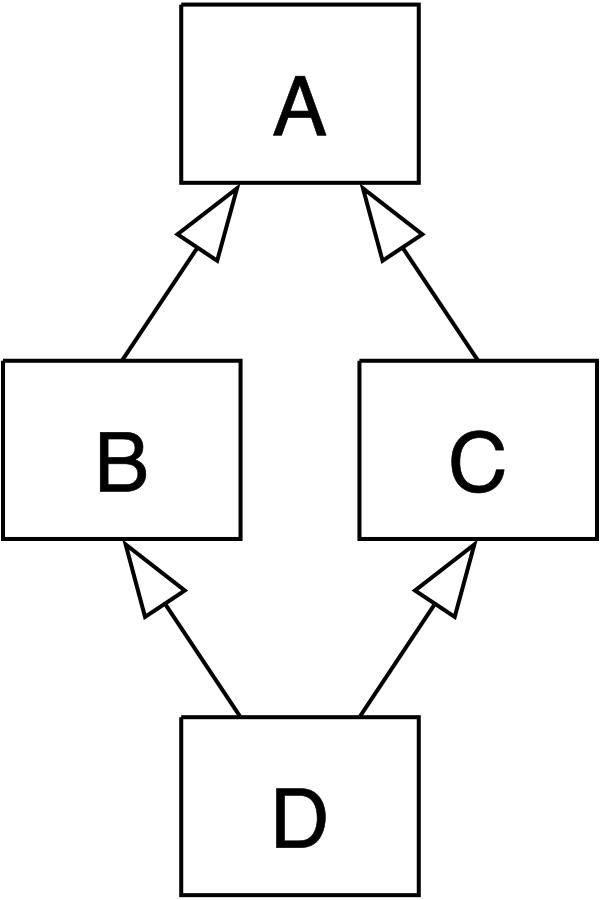
\includegraphics[width=0.15\textwidth]{diamond.png}
    \end{center}
\end{wrapfigure}
\textbf{Проблема алмаза} (diamond problem) — неопределенность, возникающая, когда два класса B и C наследуют от A, а класс D наследует от обоих классов B и C. Если метод класса D вызывает метод, определенный в классе A (и этот метод не был переопределен), а классы B и C по-своему переопределили этот метод, то тогда возникает вопрос — от какого класса его наследовать: B или C?

В \texttt{python}, в таком случае, используется алгоритм поиска в ширину. То есть, если D сначала наследуется от B, а потом от C, тогда список поиска метода в классах будет B, C, A.

\section{Работа с SQLite}%
\label{sec:Работа с SQLite}

\textbf{SQLite} — это библиотека, реализующая легковесную дисковую БД, не требующую отдельного серверного процесса и позволяющую получить доступ к БД с использованием языка запросов SQL.

Python имеет встроенную поддержку SQLite: достаточно импортировать модуль \texttt{sqlite3}.

\textbf{Основные операции при работе с БД}:
\begin{enumerate}
    \item загрузка библиотеки;
    \item создание и соединение с БД;
    \item создание таблицы БД;
    \item добавление данных;
    \item запросы на получение данных;
    \item обновление данных;
    \item удаление данных.
\end{enumerate}

\textbf{Пример работы с SQLite}:
\inputminted{python}{./examples/sqlite_conn.py}

\end{document}
